\section{Contenedor para actividades de ciencia de datos basado en R}

\subsection{Descripción}

Contenedor partiendo de una imagen base de Ubuntu al que se le añade R con distintos paquetes de ciencia de datos, concretamente:
\begin{itemize}
    \item tidyverse
    \item caret
    \item RSNNS
    \item frbs 
    \item FSinR 
    \item forecast
\end{itemize}

\subsection{Archivo Dockerfile}

\begin{figure}[H]\center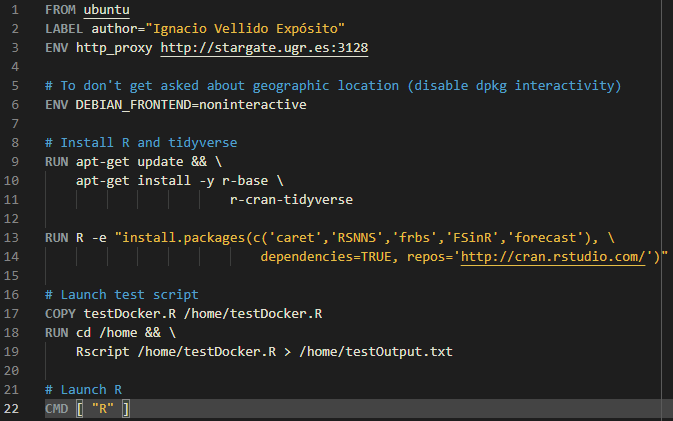
\includegraphics[width=.95\linewidth]{img/r/r0.png}\caption{}\end{figure}

El paquete ``tidyverse'' es necesario instalarlo a través de apt-get para evitar errores. 
Se incluye el proceso de testeo dentro del dockerfile para agilizar las pruebas, y se concluye indicando el comando por defecto de ejecución del script.

\subsection{Proceso de construcción}

\subsubsection{En hadoop.ugr.es}

\begin{figure}[H]\center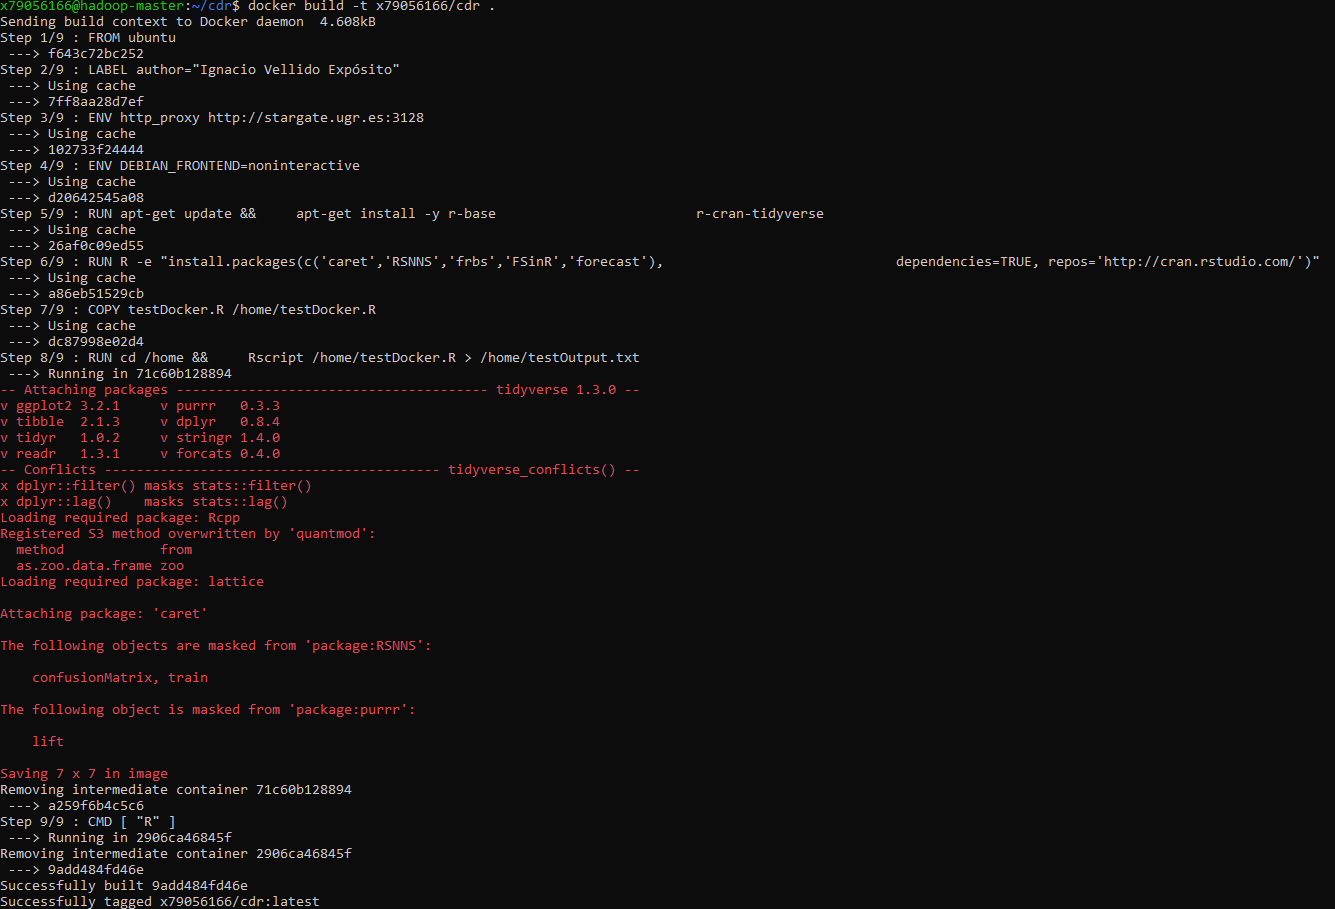
\includegraphics[width=.95\linewidth]{img/r/r1.png}\caption{Construcción de la imagen.}\end{figure}

\begin{figure}[H]\center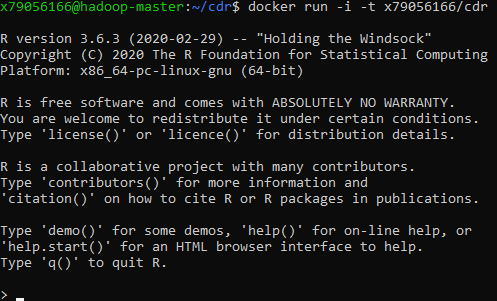
\includegraphics[width=.95\linewidth]{img/r/r3.png}\caption{Lanzando la imagen.}\end{figure}

\begin{figure}[H]\center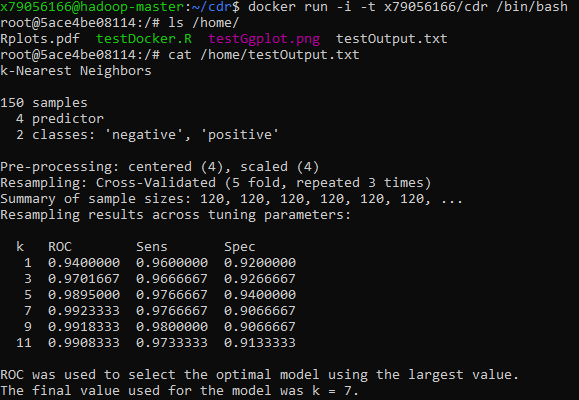
\includegraphics[width=.95\linewidth]{img/r/r2.png}\caption{Contenido de la imagen.}\end{figure}

\begin{figure}[H]\center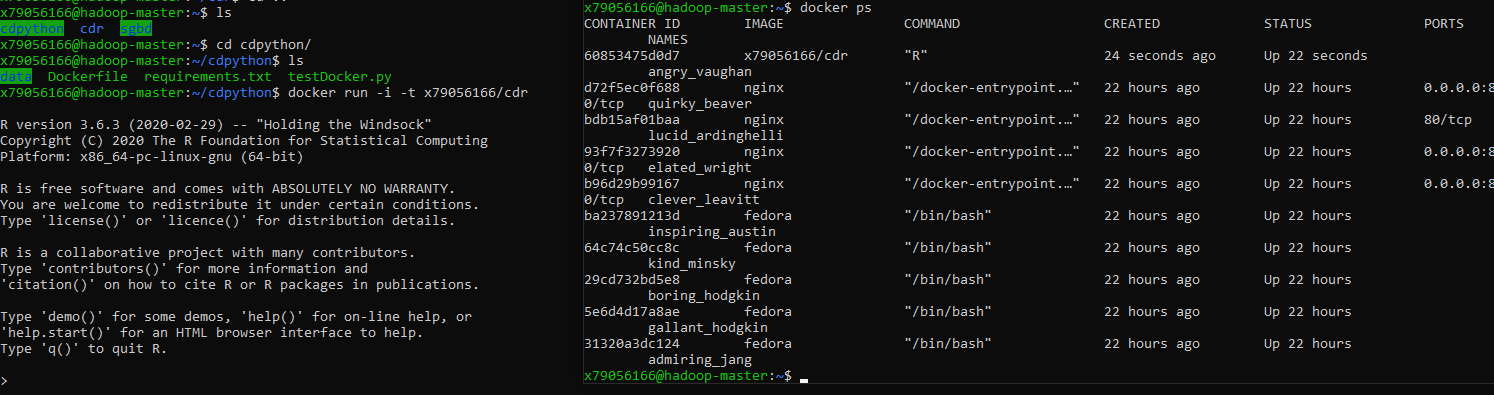
\includegraphics[width=.95\linewidth]{img/r/r4.png}\caption{Comprobando ejecución.}\end{figure}

\subsubsection{En Azure}

Tal y como está el archivo Dockerfile, si se desplegara en Azure se crearía una ``container instance'' que cargaría la imagen ejecutando el script, y se cerraría inmediatamente. Para poder acceder al contenedor antes de que se cierre, es necesario lanzar algún servicio que se mantenga en ejecutando/espera. Una opción sería desplegar una app web como Django o Flask, pero por simplicidad lanzaremos el comando indicado en \url{https://docs.microsoft.com/en-us/azure/container-instances/container-instances-troubleshooting#issues-during-container-group-runtime}

\begin{figure}[H]\center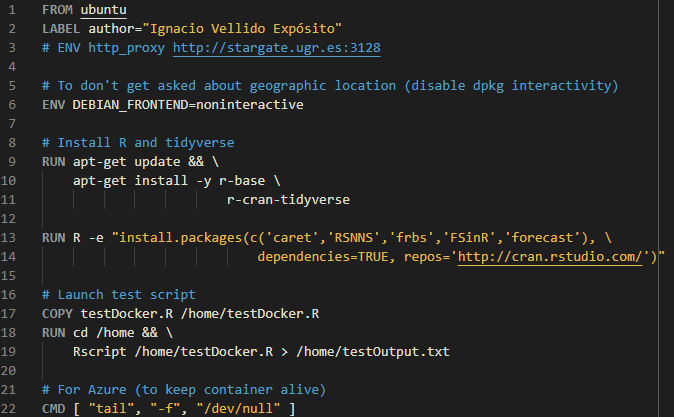
\includegraphics[width=.95\linewidth]{img/r/r11.png}\caption{Dockerfile modificado.}\end{figure}

Para hacer el despliegue, primeramente se crea un repositorio privado en Docker Hub, y se le cambia el nombre a la imagen de hadoop para adaptarla al repositorio.

\begin{figure}[H]\center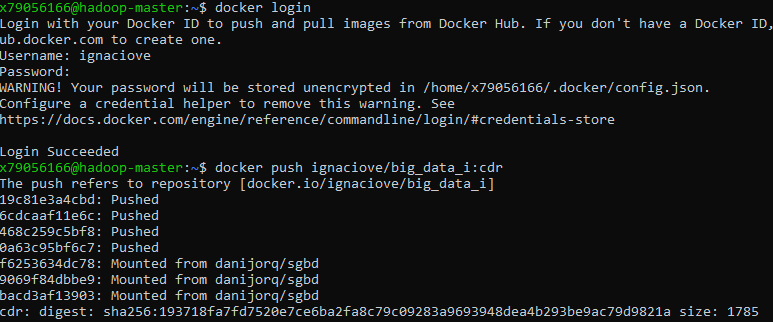
\includegraphics[width=.95\linewidth]{img/r/r5.png}\caption{Subiendo imagen al repositorio.}\end{figure}
\begin{figure}[H]\center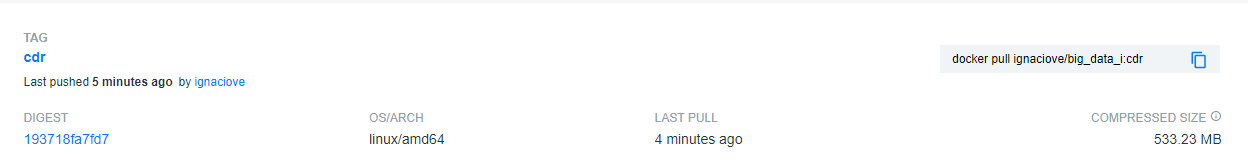
\includegraphics[width=.95\linewidth]{img/r/r6.png}\caption{Imagen en Docker Hub.}\end{figure}
\begin{figure}[H]\center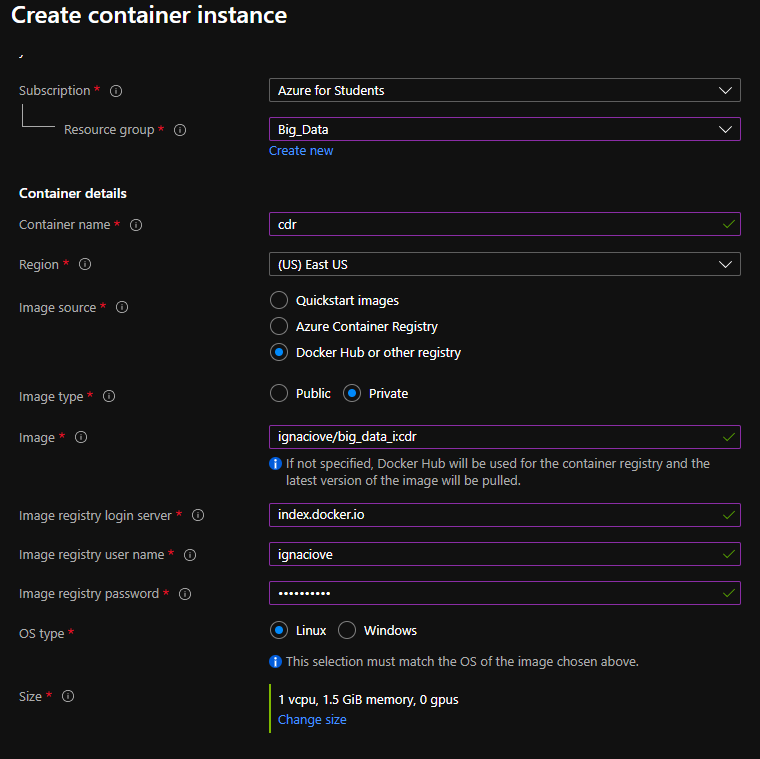
\includegraphics[width=.95\linewidth]{img/r/r7.png}\caption{Desplegando el contenedor en Azure.}\end{figure}

\begin{figure}[H]\center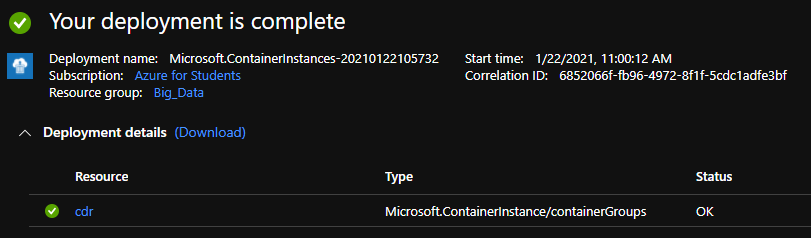
\includegraphics[width=.95\linewidth]{img/r/r8.png}\caption{Desplegando el contenedor en Azure.}\end{figure}

\begin{figure}[H]\center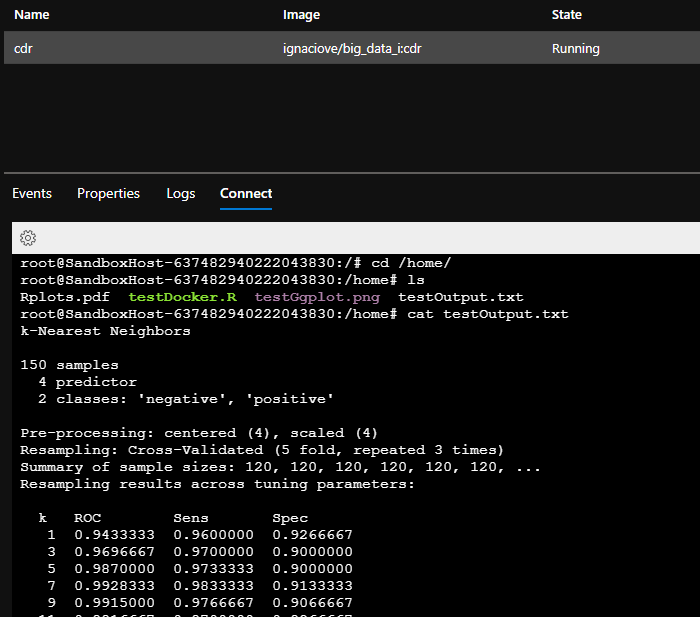
\includegraphics[width=.95\linewidth]{img/r/r10.png}\caption{Contenedor en ejecución.}\end{figure}

\subsection{Evaluación}

Para evaluar el contenedor en ambas plataformas se ha comprobado la salida del scripts. En este script se cargan todas las bibliotecas adicionales instaladas y se aplican operaciones con algunas de ellas.

\begin{figure}[H]\center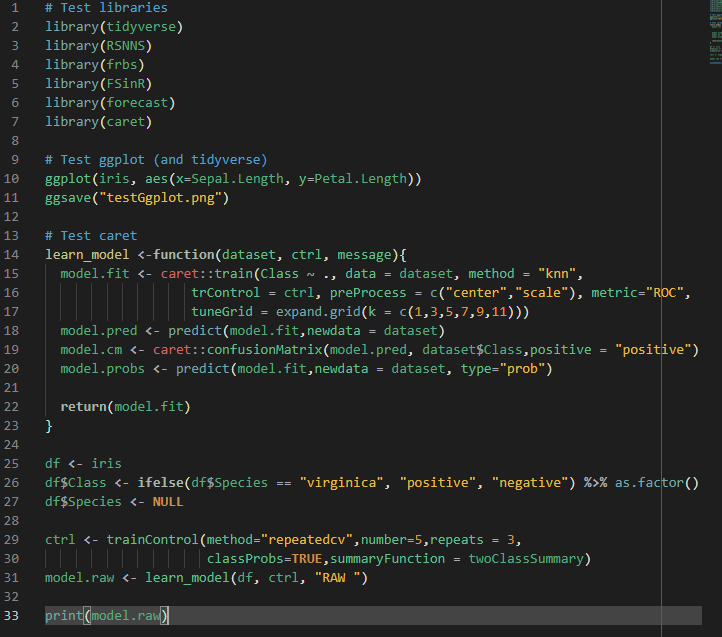
\includegraphics[width=.95\linewidth]{img/r/r9.png}\caption{Script de prueba.}\end{figure}